%============================================================================
\chapter{System architecture}
%============================================================================

\section{Components}
%============================================================================
OpenCms is a client server application that can be used in HTTP-based
environments such as the Internet. OpenCms is a classic web application
with a 3-tier-architecture (figure~\ref {3-tier1}).

\begin{figure}
\begin{center}
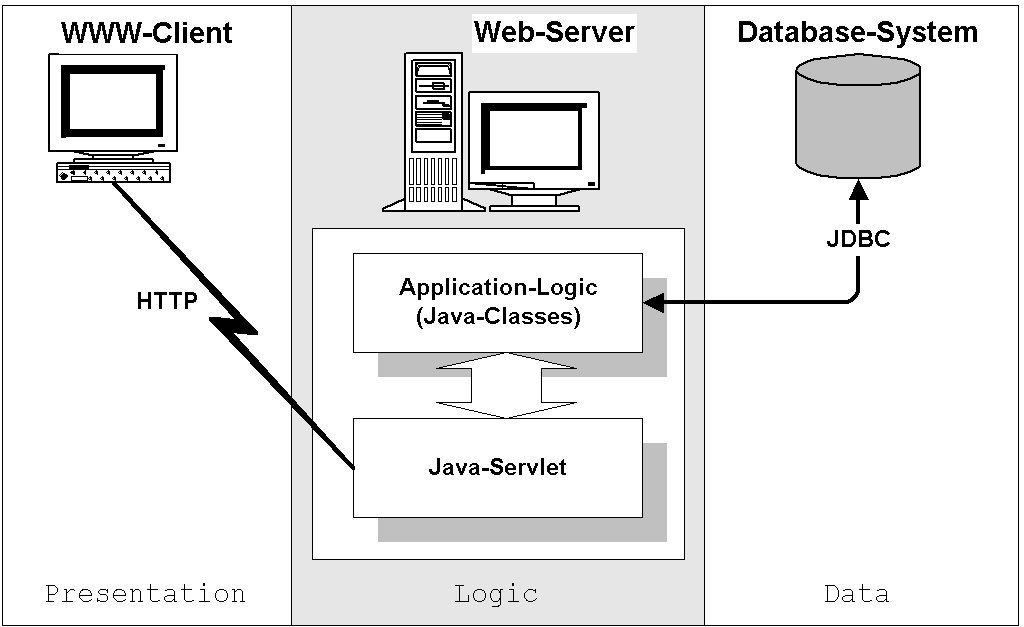
\includegraphics[clip,width=\sgw]{pics/modules/1}
\end{center}
\caption[3-tier-achitecture]{Example of a 3-tier-architecture using OpenCms}
\label{3-tier1}
\end{figure}

The presentation layer consists of a web browser (Internet Explorer or
Netscape Navigator) that is used to display and navigate through the HTML
user interface. You need a state of the art browser to use the workplace 
of OpenCms. If you use an older version of the browser you will not be able
to execute the existing DHTML functions (JavaScript code) or attach
external style sheets. Both are necessary for a correct  usage of the
application.

The logic layer lies on the web server, which is extended by a runtime
environment for Java servlets. The web server can be the Apache web
server (Version 1.3.6 or higher), the configuration of which must be
completed by the so called "Jserv module" (the Servlet Engine,
Version 1.0 or higher), in order to execute servlets. All Java classes
are installed in the servlet environment on the server.
The OpenCms servlet (one single class) provides the interface to the
presentation layer as well as the interface to the database layer. It
uses the HTTP protocol to establish the communication between the
client and the application on the server (in this case OpenCms).
The database is accessed through the JDBC interface. The database
contains tables for resource, user and property data.

The following figure shows the most important components of OpenCms 
(Figure~\ref {Components}).\\

\begin{figure}
\begin{center}
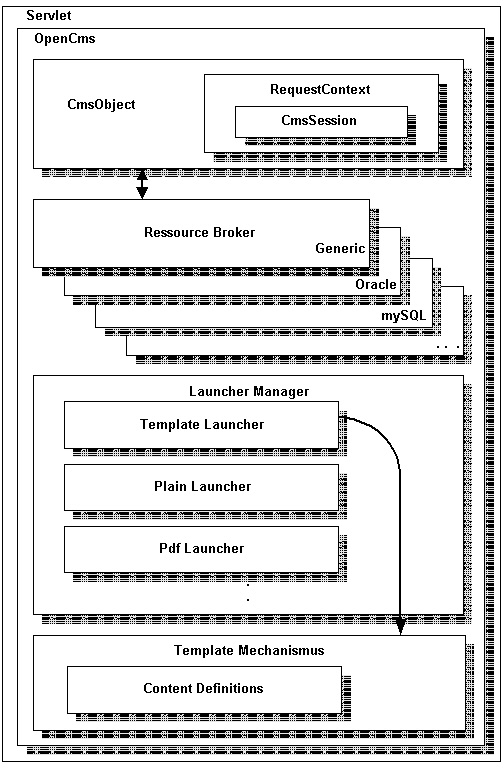
\includegraphics[clip,width=0.7 \linewidth]{pics/modules/2}
\end{center}
\caption[Components]{Compoments}
\label{Components}
\end{figure}


{\bf CmsObject:}
All resources are accessed via the \index{CmsObject} CmsObject. This is the interface to
the OpenCms system for the Module Developer. The CmsObject is
initialized with the user data.

{\bf Resource Broker:}
The \index{resource broker} resource broker checks requests for resources and performs them if
the user has the appropriate access permissions. It's configuration
depends on the database that is used.

{\bf Launcher Manager:}
The \index{Launcher Manager} Launcher Manager determines the launcher that will generate the
output with the requested content based on the type and/or content of
the selected file. If the template launcher has been selected, the
Template Mechanism is started.

{\bf Template Mechanism:}
The \index{Template Mechanism} Template Mechanism creates HTML pages based on the content in its
structured form. Content definitions enable you to access content that
originates from different sources (e.g. Virtual File System (VFS),
database, file system ...).


\section{Accessing system resources}
%============================================================================
The general procedure of requesting an OpenCms web page is shown in the
next figure. First, a request is sent from the web browser. The URL
contains the host, the servlet path and the URI. The web server starts
the \index{servlet engine} servlet engine because the URI is within the servlet path, enabling
the servlet engine to pass it to OpenCms (Figure~\ref {Accessing1}).

\begin{figure}
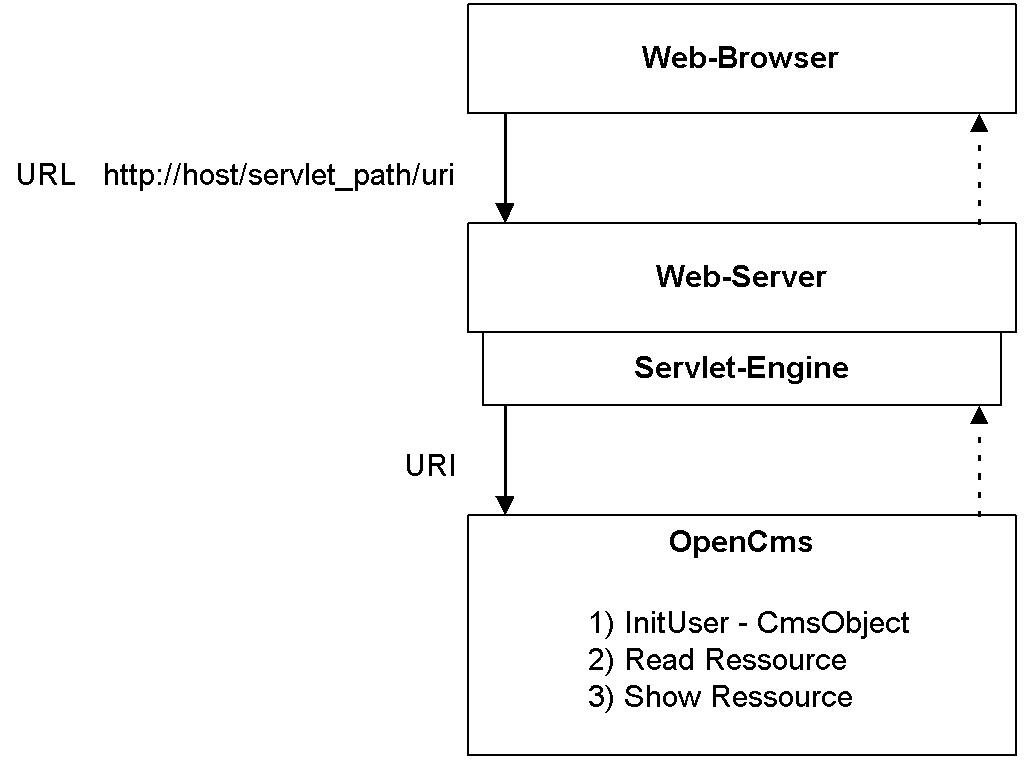
\includegraphics[clip,width=\sgw]{pics/modules/3}
\caption[Accessing system resources]{Accessing system resources}
\label{Accessing1}
\end{figure}

System resources are accessed via an instance of the class {\name CmsObject},
which provides the public interface that is used to access the system
and create the corresponding context. From the {\name msObject}, requests are
forwarded to the non-public parts of OpenCms. Thus, an instance of the
class {\name CmsObject} is created and initialized with the current user first.
The{\name CmsObject} passes the resource request to the resource broker. The
{\name resource broker} is the interface to the database. It performs the
request via the database access module and returns the resource if the
user has the right to access it. The access module establishes the
connection between the logic layer (application) and the database layer.
If a resource is requested, the {\name resource broker} forwards the request to
the access module. The access module generates an SQL statement to get
the data from the database. It then generates a {\name CmsRessourcObject} from
the database data and returns it to the resource broker. The {\name resource
broker} can now check the access permissions of the file and return the
file to the {\name CmsObject} providing the user has the appropriate access
permissions.

Because OpenCms works with different kinds of databases, the {\name resource
broker} and the access module are configured according to the used
database (Oracle, mySQL, etc.).
\index{database}
The following figure shows the structure used to access resources (figure~\ref {Accessing2}).

\begin{figure}
\begin{center}
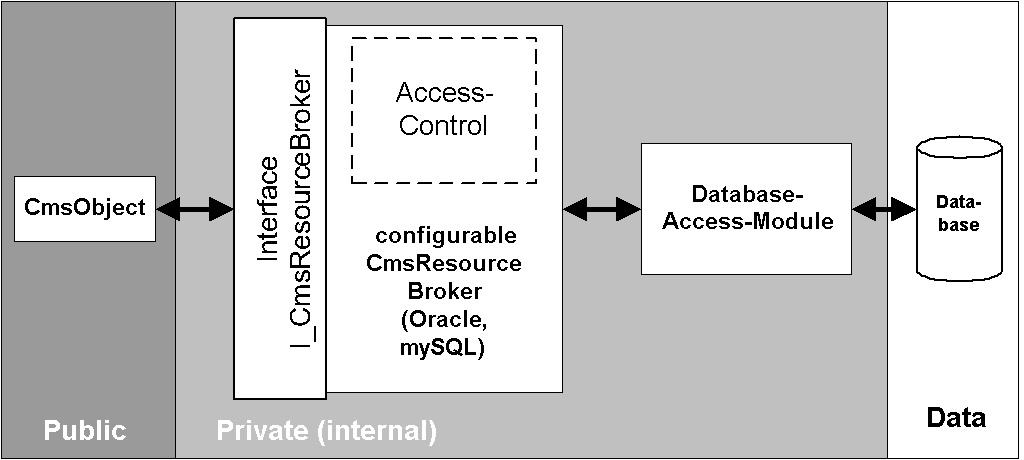
\includegraphics[clip,width=\sgw]{pics/modules/4}
\end{center}
\caption[Accessing resources in OpenCms]{Accessing resources in OpenCms}
\label{Accessing2}
\end{figure}

If the operation is successful (i.e. the user has permission to read
the file), the resource is displayed (sent to the user's web browser).

This is done by the {\name Launcher Manager}. The {\name Launcher Manager} starts a
certain launcher according to the type of the requested resource. For
pure text files, images etc. the plain launcher is used, which forwards
the content of the resource directly. The {\name template launcher} is used to
start the Template Mechanism when a template is requested. The {\name Template
Mechanism} creates HTML pages based on the content in its structured form.

The different launchers and the {\name Template Mechanism} will be explained in
detail in the following chapters.
\newpage

\section{Resources}
%============================================================================
All of the Objects that are administrated in OpenCms are called
{\name resources}. At the moment, there are eight different types of
resources. With the exception of the resource type {\name folder,} all other
types are resources files that have content that can be displayed in a
browser. The  resource type is used to provide every file with aresources
processing instance - called {\name Launcher} - which starts the processing
process and then displays the data. The following table shows the
existing relationships. {Table~\ref {resources}}
\index{resource type}
\begin{table}[h]
\begin{center}
\begin{tabular}{|l|c|p{0.50\linewidth}|l|}
\hline
{\bf Name}& 
{\bf ID}& 
{\bf Description}& 
{\bf Launcher}\\ \hline
folder&
0& Folder&none\\ \hline
plain&
1&
Files that are not processed by OpenCms (text files, JavaScript libraries etc.)&
Dump launcher\\ \hline
XMLTemplate&
2&
XML coded template file.&
XML launcher\\ \hline
page&
3&
Representation of a whole site ("clickable file" or "page file").&
XML launcher\\ \hline
binary&
4& 
Binary files (like zip archives and PDF documents, but not graphics) that can be uploaded.&
Dump launcher\\ \hline
image& 
5& 
Binary graphic files (like  GIFJPEG& 
Dump launcher\\ \hline
script& 
6& 
Designed for JavaScript on the server- side& 
Dump launcher\\ \hline
newspage&
7& 
Representation of a news article, special case of a page file& 
XML launcher\\ \hline 
JSP&
8& 
Java Server Page& 
JSP loader\\ \hline 
\end{tabular}
\caption [Resources in OpenCms]{Resources in OpenCms}
\end{center}
\label{resources}
\end{table}

\section{The Virtual File System (VFS) of OpenCms}
\index{Virtual File System}
\index{VFS}
All of the files and folders of the different projects that are
displayed in the Explorer view that is part of the OpenCms Workplace,
are not stored in the normal file system. OpenCms has a {\name Virtual File
System} that holds the files and folders in a database, and an integrated
access permission administration. The access permissions in OpenCms are
similar to those of the UNIX file system. However, by using a {\name VFS} and a
database, OpenCms is independent from the operating system that is
installed on the server. In this way OpenCms can run on a Windows 95/98
system, which itself has no access permission administration at all.
Here is a short overview of the folders and the files in the standard
OpenCms {\name Virtual File System:} {Table~\ref {VFS}}

\begin{table}[!h]
\begin{center}
\begin{tabular}{|l|p{0.55\linewidth}|}
\hline
{\bf Directory}&
{\bf Files located in the directory}\\ [0.5ex] \hline

{\dir /system}&
Parent directory of the directories that contain workplace templates and configuration files for the system.\\ \hline

{\dir /system/bodies}&
Body templates are stored in this directory or a subdirectory thereof. They are stored in a directory with the same name
as the directory in which the web site is located.\\ \hline

{\dir /system/modules}&
OpenCms modules are automatically placed below this directory.\\ \hline

{\dir /system/modules/default}&
Location of the default module which contains a basic empty template and some resource files.\\ \hline

{\dir /system/modules/default/templates}&
The default master templates that define the general layout of a web site.\\ \hline

{\dir /system/galleries}&
Basis location of all galleries that are available in the editor.\\ \hline

{\dir /system/galleries/download}&
Gallery for files that can be downloaded.\\ \hline

{\dir /system/galleries/pics}&
Gallery for pictures that are used in web sites.\\ \hline

{\dir /system/login}&
The OpenCms workplace login screen in located here.\\ \hline

{\dir /system/workplace}&
The OpenCms workplace application files are located in this subdirectory.\\ \hline

{\dir /system/workplace/action}&
Executable files like login, copy etc.\\ \hline

{\dir /system/workplace/templates}&
The templates that are used to create the workplace.\\ \hline

{\dir /system/workplace/scripts}&
Javascript files used in the workplace are placed here.\\ \hline

{\dir /system/workplace/administration}&
Subdirectories for every Item in the Administration view.\\ \hline

{\dir /system/workplace/locales}&
The workplace locales, i.e. language files reside here. 
They are stored in a separate subdirectory for every language.\\ \hline

{\dir /system/workplace/resources}&
Workplace static resources are placed in this directory.
These are the style sheets used and the images for system elements like buttons etc.\\ \hline

{\dir /system/workplace/help}&
The help system.\\ \hline

\end{tabular}
\caption [VFS of OpenCms]{VFS of OpenCms}
\end{center}
\label{VFS}
\end{table}

Please note that the VFS structure was modified in the 5.0 release of OpenCms.
Previous versions had a layout different from the one described above.

\section{Class structure}
%============================================================================
The functionality of OpenCms is implemented in many different Java
classes. The classes are divided into different packages to structure
the code. Currently, there are 10 packages that  cover a certain part
of the system's functionality. {Table~\ref {Classtruc}}

\begin{table}[!h]
\begin{center}
\begin{tabular}{|l|p{0.55\linewidth}|}
\hline
{\name com.opencms.core}&
Classes of the system's core. The package also contains the OpenCms servlet.\\ \hline
{\name com.opencms.file}&
Definitions of all of the objects. \\ \hline
{\name com.opencms.file.genericSql}&
Resource broker for generic SQL databases. \\ \hline
{\name com.opencms.file.mySql}&
Special resource broker for mySQL.\\ \hline
{\name  com.opencms.file.oracleplsql}&
Special resource broker for ORACLE.\\ \hline
{\name com.opencms.file.utils}&
File package.\\ \hline
{\name com.opencms.launcher}&
All of the launchers that are used to display files or templates and a Launcher Manager.\\ \hline
{\name com.opencms.template}&
All of the template classes that are used to create documents dynamically and a Template Manager.\\ \hline
{\name com.opencms.util}&
Some general functionality (encoder, decoder etc.)\\ \hline
{\name com.opencms.workplace}&
All of the components (e.g. buttons, context-sensitive menus etc.) and functions (e.g. create project) of
the user interface (OpenCms Workplace).\\ \hline

\end{tabular}
\caption [Class structure]{Class structure}
\label {Classtruc}
\end{center}
\end{table}